%        File: SailingOverview.tex
%     Created: Fri Nov 18 11:00 AM 2011 E
% Last Change: Fri Nov 18 11:00 AM 2011 E
%
\documentclass[letterpaper]{article}
\usepackage{graphicx} % For figures and images
\usepackage{alltt} % For better verbatim
\usepackage[]{hyperref} % Links
\usepackage[]{url} % External Links
\usepackage{setspace}
\usepackage{fancyvrb}
\usepackage{color}
\usepackage[ascii]{inputenc}

% The HRule command is required for the title page
% from the wikibook
\newcommand{\HRule}{\rule{\linewidth}{0.5mm}}

% Change the paragraphs to block style
\setlength{\parindent}{0pt}
\setlength{\parskip}{2ex}

\begin{document}
\makeatletter
\def\PY@reset{\let\PY@it=\relax \let\PY@bf=\relax%
    \let\PY@ul=\relax \let\PY@tc=\relax%
    \let\PY@bc=\relax \let\PY@ff=\relax}
\def\PY@tok#1{\csname PY@tok@#1\endcsname}
\def\PY@toks#1+{\ifx\relax#1\empty\else%
    \PY@tok{#1}\expandafter\PY@toks\fi}
\def\PY@do#1{\PY@bc{\PY@tc{\PY@ul{%
    \PY@it{\PY@bf{\PY@ff{#1}}}}}}}
\def\PY#1#2{\PY@reset\PY@toks#1+\relax+\PY@do{#2}}

\def\PY@tok@gd{\def\PY@tc##1{\textcolor[rgb]{0.63,0.00,0.00}{##1}}}
\def\PY@tok@gu{\let\PY@bf=\textbf\def\PY@tc##1{\textcolor[rgb]{0.50,0.00,0.50}{##1}}}
\def\PY@tok@gt{\def\PY@tc##1{\textcolor[rgb]{0.00,0.25,0.82}{##1}}}
\def\PY@tok@gs{\let\PY@bf=\textbf}
\def\PY@tok@gr{\def\PY@tc##1{\textcolor[rgb]{1.00,0.00,0.00}{##1}}}
\def\PY@tok@cm{\let\PY@it=\textit\def\PY@tc##1{\textcolor[rgb]{0.25,0.50,0.50}{##1}}}
\def\PY@tok@vg{\def\PY@tc##1{\textcolor[rgb]{0.10,0.09,0.49}{##1}}}
\def\PY@tok@m{\def\PY@tc##1{\textcolor[rgb]{0.40,0.40,0.40}{##1}}}
\def\PY@tok@mh{\def\PY@tc##1{\textcolor[rgb]{0.40,0.40,0.40}{##1}}}
\def\PY@tok@go{\def\PY@tc##1{\textcolor[rgb]{0.50,0.50,0.50}{##1}}}
\def\PY@tok@ge{\let\PY@it=\textit}
\def\PY@tok@vc{\def\PY@tc##1{\textcolor[rgb]{0.10,0.09,0.49}{##1}}}
\def\PY@tok@il{\def\PY@tc##1{\textcolor[rgb]{0.40,0.40,0.40}{##1}}}
\def\PY@tok@cs{\let\PY@it=\textit\def\PY@tc##1{\textcolor[rgb]{0.25,0.50,0.50}{##1}}}
\def\PY@tok@cp{\def\PY@tc##1{\textcolor[rgb]{0.74,0.48,0.00}{##1}}}
\def\PY@tok@gi{\def\PY@tc##1{\textcolor[rgb]{0.00,0.63,0.00}{##1}}}
\def\PY@tok@gh{\let\PY@bf=\textbf\def\PY@tc##1{\textcolor[rgb]{0.00,0.00,0.50}{##1}}}
\def\PY@tok@ni{\let\PY@bf=\textbf\def\PY@tc##1{\textcolor[rgb]{0.60,0.60,0.60}{##1}}}
\def\PY@tok@nl{\def\PY@tc##1{\textcolor[rgb]{0.63,0.63,0.00}{##1}}}
\def\PY@tok@nn{\let\PY@bf=\textbf\def\PY@tc##1{\textcolor[rgb]{0.00,0.00,1.00}{##1}}}
\def\PY@tok@no{\def\PY@tc##1{\textcolor[rgb]{0.53,0.00,0.00}{##1}}}
\def\PY@tok@na{\def\PY@tc##1{\textcolor[rgb]{0.49,0.56,0.16}{##1}}}
\def\PY@tok@nb{\def\PY@tc##1{\textcolor[rgb]{0.00,0.50,0.00}{##1}}}
\def\PY@tok@nc{\let\PY@bf=\textbf\def\PY@tc##1{\textcolor[rgb]{0.00,0.00,1.00}{##1}}}
\def\PY@tok@nd{\def\PY@tc##1{\textcolor[rgb]{0.67,0.13,1.00}{##1}}}
\def\PY@tok@ne{\let\PY@bf=\textbf\def\PY@tc##1{\textcolor[rgb]{0.82,0.25,0.23}{##1}}}
\def\PY@tok@nf{\def\PY@tc##1{\textcolor[rgb]{0.00,0.00,1.00}{##1}}}
\def\PY@tok@si{\let\PY@bf=\textbf\def\PY@tc##1{\textcolor[rgb]{0.73,0.40,0.53}{##1}}}
\def\PY@tok@s2{\def\PY@tc##1{\textcolor[rgb]{0.73,0.13,0.13}{##1}}}
\def\PY@tok@vi{\def\PY@tc##1{\textcolor[rgb]{0.10,0.09,0.49}{##1}}}
\def\PY@tok@nt{\let\PY@bf=\textbf\def\PY@tc##1{\textcolor[rgb]{0.00,0.50,0.00}{##1}}}
\def\PY@tok@nv{\def\PY@tc##1{\textcolor[rgb]{0.10,0.09,0.49}{##1}}}
\def\PY@tok@s1{\def\PY@tc##1{\textcolor[rgb]{0.73,0.13,0.13}{##1}}}
\def\PY@tok@sh{\def\PY@tc##1{\textcolor[rgb]{0.73,0.13,0.13}{##1}}}
\def\PY@tok@sc{\def\PY@tc##1{\textcolor[rgb]{0.73,0.13,0.13}{##1}}}
\def\PY@tok@sx{\def\PY@tc##1{\textcolor[rgb]{0.00,0.50,0.00}{##1}}}
\def\PY@tok@bp{\def\PY@tc##1{\textcolor[rgb]{0.00,0.50,0.00}{##1}}}
\def\PY@tok@c1{\let\PY@it=\textit\def\PY@tc##1{\textcolor[rgb]{0.25,0.50,0.50}{##1}}}
\def\PY@tok@kc{\let\PY@bf=\textbf\def\PY@tc##1{\textcolor[rgb]{0.00,0.50,0.00}{##1}}}
\def\PY@tok@c{\let\PY@it=\textit\def\PY@tc##1{\textcolor[rgb]{0.25,0.50,0.50}{##1}}}
\def\PY@tok@mf{\def\PY@tc##1{\textcolor[rgb]{0.40,0.40,0.40}{##1}}}
\def\PY@tok@err{\def\PY@bc##1{\fcolorbox[rgb]{1.00,0.00,0.00}{1,1,1}{##1}}}
\def\PY@tok@kd{\let\PY@bf=\textbf\def\PY@tc##1{\textcolor[rgb]{0.00,0.50,0.00}{##1}}}
\def\PY@tok@ss{\def\PY@tc##1{\textcolor[rgb]{0.10,0.09,0.49}{##1}}}
\def\PY@tok@sr{\def\PY@tc##1{\textcolor[rgb]{0.73,0.40,0.53}{##1}}}
\def\PY@tok@mo{\def\PY@tc##1{\textcolor[rgb]{0.40,0.40,0.40}{##1}}}
\def\PY@tok@kn{\let\PY@bf=\textbf\def\PY@tc##1{\textcolor[rgb]{0.00,0.50,0.00}{##1}}}
\def\PY@tok@mi{\def\PY@tc##1{\textcolor[rgb]{0.40,0.40,0.40}{##1}}}
\def\PY@tok@gp{\let\PY@bf=\textbf\def\PY@tc##1{\textcolor[rgb]{0.00,0.00,0.50}{##1}}}
\def\PY@tok@o{\def\PY@tc##1{\textcolor[rgb]{0.40,0.40,0.40}{##1}}}
\def\PY@tok@kr{\let\PY@bf=\textbf\def\PY@tc##1{\textcolor[rgb]{0.00,0.50,0.00}{##1}}}
\def\PY@tok@s{\def\PY@tc##1{\textcolor[rgb]{0.73,0.13,0.13}{##1}}}
\def\PY@tok@kp{\def\PY@tc##1{\textcolor[rgb]{0.00,0.50,0.00}{##1}}}
\def\PY@tok@w{\def\PY@tc##1{\textcolor[rgb]{0.73,0.73,0.73}{##1}}}
\def\PY@tok@kt{\def\PY@tc##1{\textcolor[rgb]{0.69,0.00,0.25}{##1}}}
\def\PY@tok@ow{\let\PY@bf=\textbf\def\PY@tc##1{\textcolor[rgb]{0.67,0.13,1.00}{##1}}}
\def\PY@tok@sb{\def\PY@tc##1{\textcolor[rgb]{0.73,0.13,0.13}{##1}}}
\def\PY@tok@k{\let\PY@bf=\textbf\def\PY@tc##1{\textcolor[rgb]{0.00,0.50,0.00}{##1}}}
\def\PY@tok@se{\let\PY@bf=\textbf\def\PY@tc##1{\textcolor[rgb]{0.73,0.40,0.13}{##1}}}
\def\PY@tok@sd{\let\PY@it=\textit\def\PY@tc##1{\textcolor[rgb]{0.73,0.13,0.13}{##1}}}

\def\PYZbs{\char`\\}
\def\PYZus{\char`\_}
\def\PYZob{\char`\{}
\def\PYZcb{\char`\}}
\def\PYZca{\char`\^}
\def\PYZsh{\char`\#}
\def\PYZpc{\char`\%}
\def\PYZdl{\char`\$}
\def\PYZti{\char`\~}
% for compatibility with earlier versions
\def\PYZat{@}
\def\PYZlb{[}
\def\PYZrb{]}
\makeatother

% If the titlepage is included, uncomment below.
%%        File: /Users/allgood38/git/newmast/Documentation/title.tex
%     Created: Fri Nov 18 11:00 am 2011 E
% Last Change: Fri Nov 18 11:00 am 2011 E
%
% The root of this document is taken from the core of the Latex
% Wikibook. Not meant to be compiled on its own, instead to be
% inserted into the document using the \input command within the
% document tags.
\begin{titlepage}

% Center all the titles and junk before the minipages begin. 
\begin{center}

% Here Graphics are normally included, if there are none use
% the command directly under it to add some space, otherwise it
% doesn't look very good.
% \includegraphics[width=0.15\textwidth]{./logo}\\[1cm]    
{\ }\\[2.2cm]
\textsc{\LARGE QMAST Sailcode}\\[1.5cm]

% A sort of subtitle under the large text
\textsc{\Large Software Guide 2011}\\[0.5cm]


% Title enclosed in horizontal lines
\HRule \\[0.4cm]
{ \huge \bfseries API Documentation}\\[0.4cm]
\HRule \\[1.5cm]
% Minipages are coming up, so stop centering.
\end{center}

% The Minipage on the left-hand side
\begin{raggedright}
\begin{minipage}{0.4\textwidth}
% Insert Author/Group info here
\begin{flushleft} \large
Stephen Cripps \\
			9skc@queensu.ca \\
			06141178
			\end{flushleft}
			% End of the Author/Group info
			\end{minipage}
			\end{raggedright}

			% Space for the right-hand side minipage, note that it
			% doesn't work with long names/lines.
			%\begin{minipage}{0.4\textwidth}
			%	% Add more stuff between the flushright commands.
			%	\begin{flushright} \large
			%	\emph{Supervisor:} \\
				%	Dr.~Mark \textsc{Brown}
				%	\end{flushright}
				%\end{minipage}

				% Fills up the space between the content and the date
				\vfill

				% Bottom of the page
				\begin{center}
{\large \today}
\end{center}


\end{titlepage}



%\doublespacing

\section{The Sailcode Application Interface} % (fold)
\label{sec:The Sailcode Application Interface}

The goal of this software rewrite is to make the code more modular. Modular code can be changed without worrying about breaking other parts of the code. Whenever a change is made to a module, we will run a \emph{unit test} to check to make sure that it performs the same operation by handling the same input and output. This way if something has been changed in such a way that it would break other parts of the code, we will know.

The new API is going to contain as much code which has already been written in an effort to save time, since a lot of work went into it which did produce some good results.

\begin{figure}[h]
	\centering
	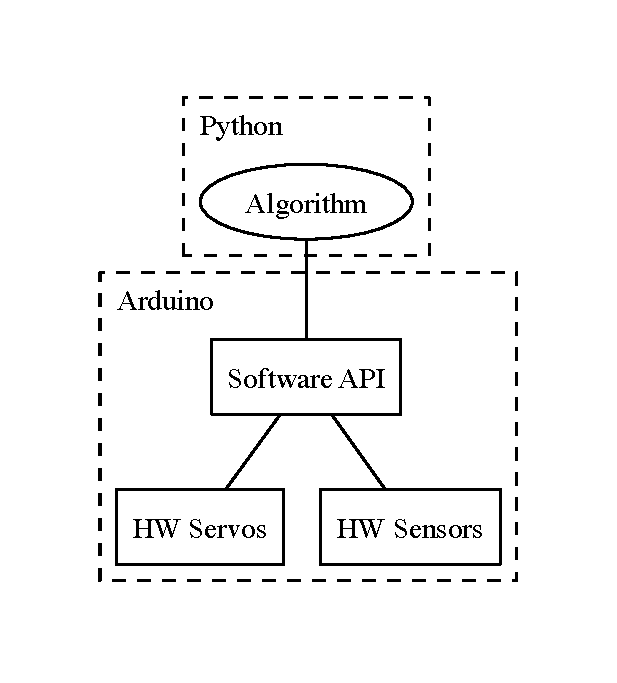
\includegraphics[width=0.4\linewidth]{mindmap_test/overview.pdf}
	\caption{Rough overview of software location}
	\label{fig:overview}
\end{figure}

% section The Sailcode Application Interface (end)

\subsection{Classes in Arduino} % (fold)
\label{sec:Classes in Arduino}

\url{http://arduino.cc/en/Hacking/LibraryTutorial}

The underlying software Arduino is built on attempts to implement the C/C++ language and is able to understand almost all of it. There are a few things that are not, such as the \verb+new+ and \verb+delete+, but there is a work around for this. The one thing it will not support, is the use of template functions. Template functions allow you to make functions that can operate on arbitrary data types, and wouldn't really be useful for our purposes anyways.

When you write a class on the Arduino, you write it in a library. Where a library is just another set of source files which are included in the build. The Arduino IDE is very picky about where you put the library files, but the eclipse IDE just requires you to have a valid include statement. Check out the link above for more info. 

% section Classes in Arduino (end)

\subsection{The Wind Sensor} % (fold)
\label{sec:The Wind Sensor}

Will be contained in its own class and carry all of its own supporting variables.

The sensor will just keep sending serial data at intervals rather than waiting for a command, so we have to have a way to keep the most recent value stored. This could mean having it update every-single time it gets a new string, then have the values ready for when a function is called, or it could ignore all messages until a function is called which requests an update of the variables.

\begin{figure}[h]
	\centering
	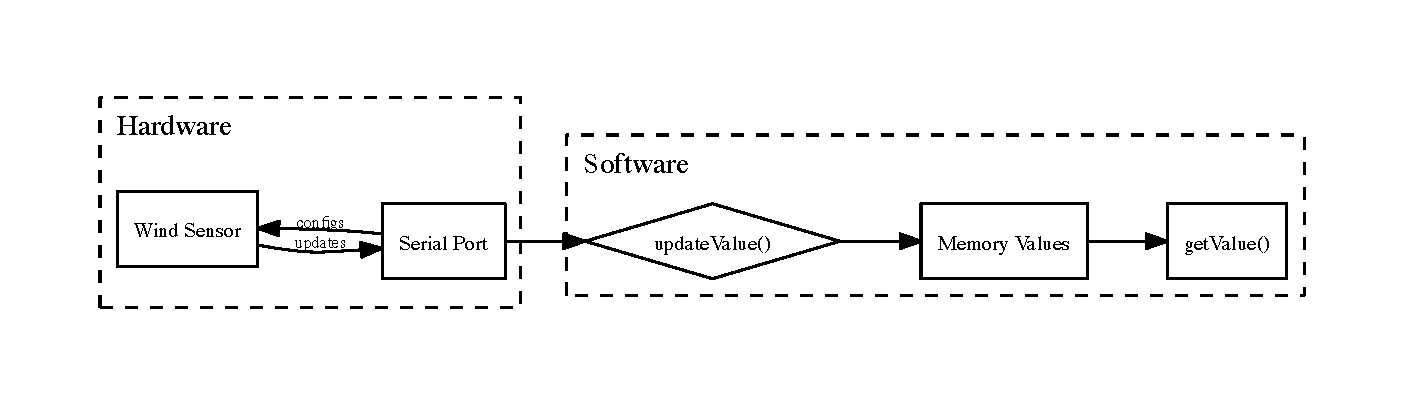
\includegraphics[width=\linewidth]{maps/WindSerial.pdf}
	\caption{Wind Sensor to Memory path}
	\label{fig:WindSensorMap}
\end{figure}

When the wind sensor is asked to update its values from the sensor, it will call the series of functions in Figure \ref{fig:newparse} in order to get the values. It just breaks up everything required to get the data from the serial buffer, isolate an NMEA sentence, parse it into values and update the local object variables.

\begin{figure}[h]
	\centering
	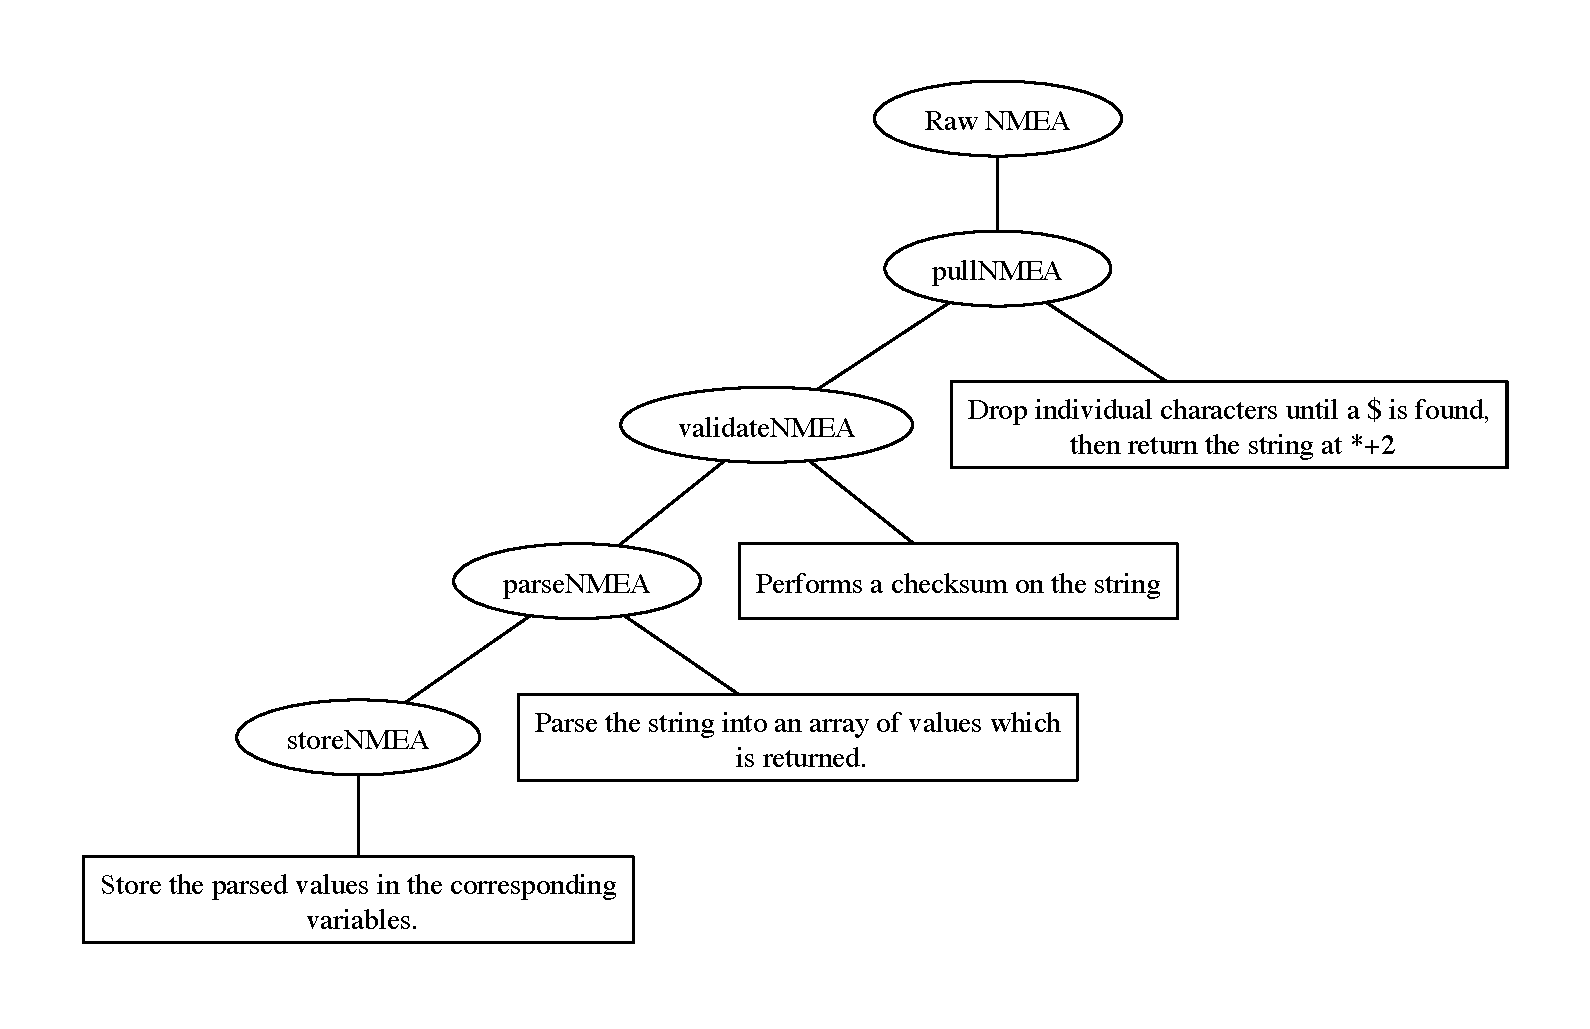
\includegraphics[width=\linewidth]{maps/newparse.pdf}
	\caption{Wind sensor algorithm}
	\label{fig:newparse}
\end{figure}

The wind sense object is going to have a variable which will store a partially completed sentence, which will continue to be completed by the pullNMEA function. Once the partial sentence is complete, it will raise a flag, and allow the validateNMEA function to operate on it. If it is valid the sentence will be passed on to the parse function, which will return an array of strings containing the isolated values. If there are two comma's, then a null value will be stored to that location. That way when the array is given to the storage function, it will be able to figure out why there are null values, and put something appropriate in its place. 

Pulling the individual characters is done by calling the \verb:grabNMEAChar: function, which accepts a single character and stores it in the \verb:partSentence: variable, but only if it starts with a \$ or if it has already started adding characters to a string. If it encounters anything else, it simply doesn't store the character. If it were reading from the serial buffer, this would also remove it from the serial buffer. 

Once the function reaches an asterisk, it stops after two more characters so that it can include the given checksum. In this manner, we have isolated an NMEA sentence which can be sent through to the next function. 

\subsection{NMEA Parsing} % (fold)
\label{sub:NMEA Parsing}

Rather than using a built-in function, the sentences will be parsed one character at a time. The built-in strtok function has the advantage in that it is so flexible, whereas this function will only be able to parse NMEA sentences. At the same time, it should be able to parse any NMEA style sentence, since all it is going to do is break the sentence into an array of character-array strings, which will be converted into the correct values in the next function, storeNMEA.

The function starts with an array of arbitrary size, which should be greater than the maximum number of possible values included in an NMEA sentence. There are three strings involved and three index variables to keep track of their progress. The first is the index for the input NMEA sentence, which be incremented with every iteration until an asterisk character is reached and the function will stop. The second string is for building a new value and also has an index to keep track of how many digits have been added to it. The third string is actually an array of strings. This is what the function will return once it has finished. The array also has an index, but this is to keep track of the number of strings which has been added to it.

The parseNMEA function is meant to return an array of strings. However, I have opted to use strings in their most basic form, as an array of characters. Initially, the idea was to use an array of char array pointers, which have malloc assign them them memory based off of the length of the value. Given the complication of assigning memory though, we will instead set the size of the array in a static way. Simply using a 2-dimensional array of type char. 

This function won't actually return an array anymore, instead it will modify a two dimensional char array which is handed to it as an argument. The declaration of the array is done in the WindSense object header file as a private member. The actual parsing of the strings isn't that tricky. The algorithm just needs to follow the decisions given in Figure \ref{fig:parsingTree}. 

Once an array of strings is created, they should contain both the identification tags for the NMEA string and the values themselves. Next the storeNMEA function will be able to take these parsed values and turn them into integer, double and char values depending on what it is.

\begin{figure}[h]
	\centering
	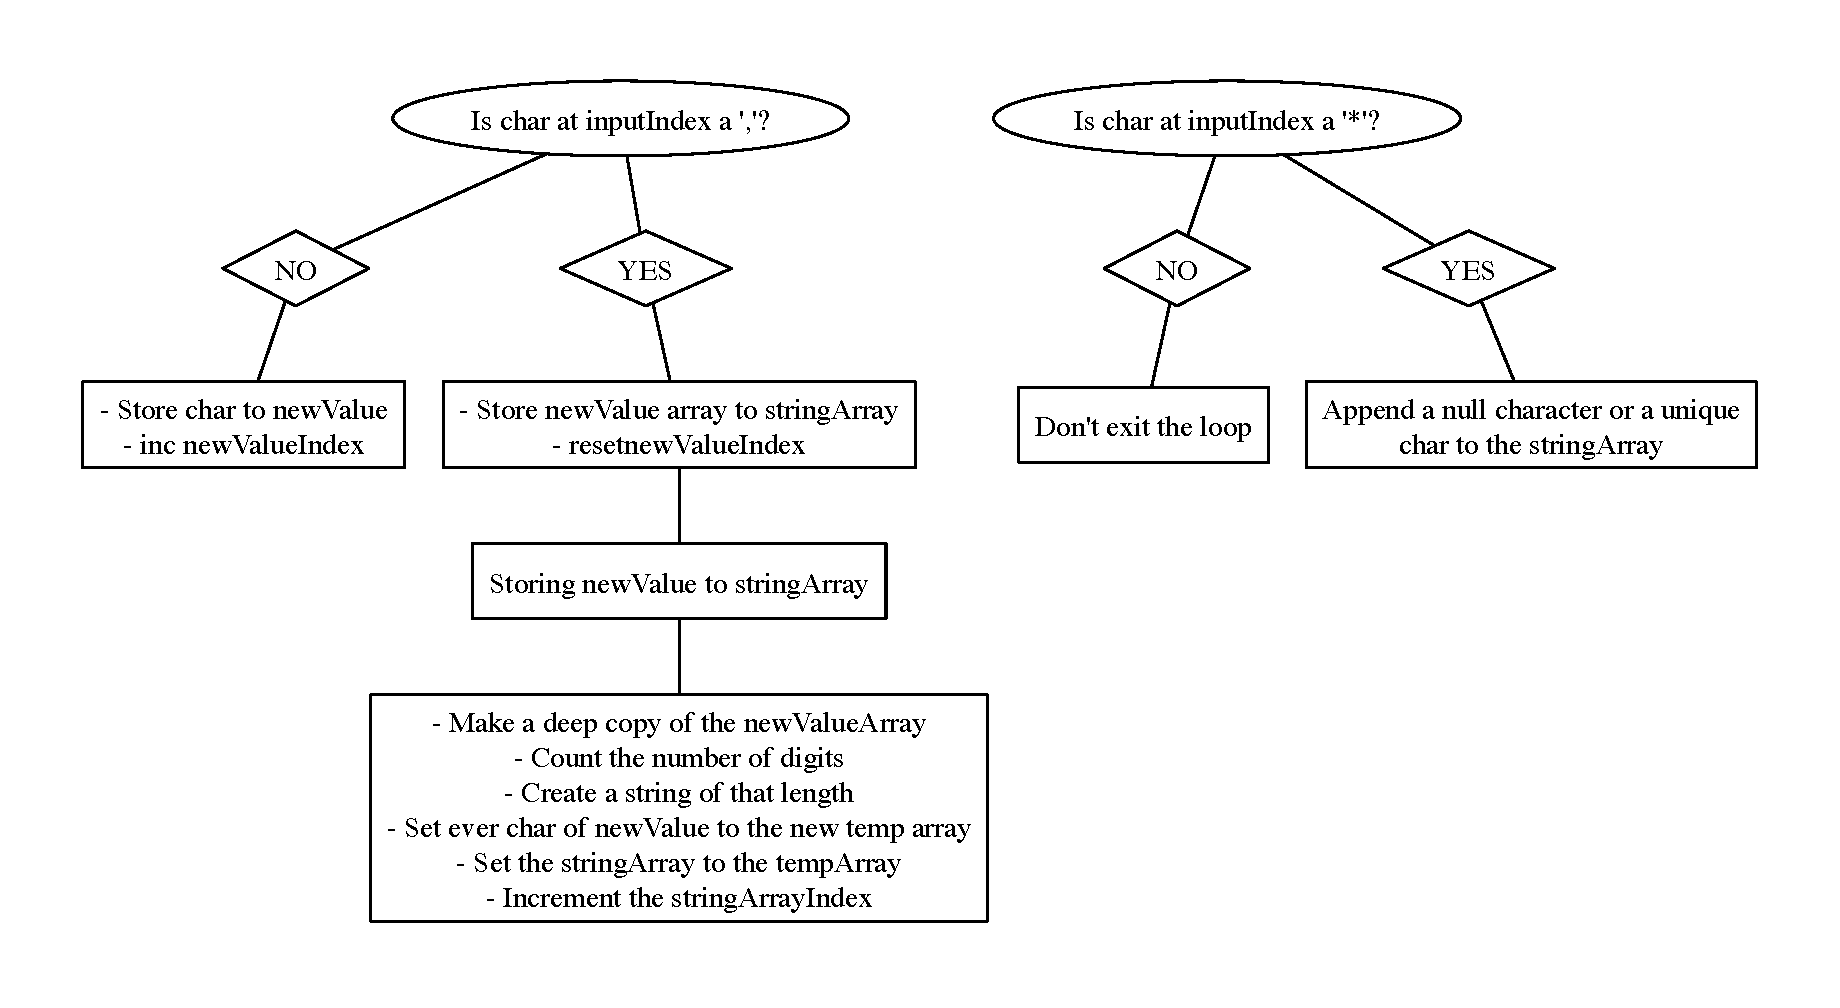
\includegraphics[width=\linewidth]{maps/parsing.pdf}
	\caption{Parsing decision tree}
	\label{fig:parsingTree}
	% TODO this diagram really sucks, but we should use something like it.
	% No detailed description will be given until a new one is made
\end{figure}

It would definitely be less memory intensive to isolate each of the string values, then update the corresponding variable in the object, but this method lends itself to being more modular. If memory does become an issue, we can switch to the other method.

The while loop which makes up the core of this function has a weird condition. It loops as long as the input index is less than or equal to 1 or if the character just before the index does not equal the '*' character. This was done to allow the loop to execute once even after the asterisk was encountered. The first condition was included to prevent the second condition from accessing a negative index value from the input string on its first iteration. This is nice because if the first condition is true, then the compiler doesn't check the second condition.

% subsection NMEA Parsing (end)

\subsection{Interfacing the Hardware} % (fold)
\label{sub:Interfacing the Hardware}

The wind sensor is connected to the Arduino through Serial port 3, which runs through the power board.

\begin{table}[h]
	\centering
	\begin{tabular}{c|c}
		\hline
		Data Rate 	& 	4800 BPS 	\\
		Commmand 	& 	\$PAMTC,EN,RMC,0,10 \\
	\end{tabular}
	\caption{Useful Specs}
	\label{tbl:windspecs}
\end{table}

% subsection Interfacing the Hardware (end)

% section The Wind Sensor (end)

\bibliographystyle{plain}
\bibliography{plans}
\nocite{*}


\begin{itemize}
	\item The wind direction relative to the front of the boat
	\item The current GPS Location of the boat
\end{itemize}
\section{Sailing Navigation} % (fold)
\label{sec:Sailing Navigation}

\subsection{Navigation with GPS Data} % (fold)
\label{sec:Navigation with GPS Data}

The boat is going to be given certain points that it needs to reach.
These will be given to it through a data file containing the GPS
locations. Given that the boat cannot sail a straight line to the
objective, it is going to need to deal with changing wind conditions and
any other obstacles.

From this point on, the locations which the robot must reach will be called
hard coded locations. In order to reach these locations, the robot will generate
a series of in between points to take care of the challenges of sailing to the
hard coded points.

% Testing the code highlighting
\begin{Verbatim}[commandchars=\\\{\}]
\PY{c+cp}{\PYZsh{}}\PY{c+cp}{include <stdio.h>}

\PY{k+kt}{int} \PY{n+nf}{main}\PY{p}{(}\PY{k+kt}{int} \PY{n}{argc}\PY{p}{,} \PY{k}{const} \PY{k+kt}{char} \PY{o}{*}\PY{n}{argv}\PY{p}{[}\PY{p}{]}\PY{p}{)}
\PY{p}{\PYZob{}}
	\PY{n}{printf}\PY{p}{(}\PY{l+s}{"}\PY{l+s}{This shit is bananas}\PY{l+s+se}{\PYZbs{}n}\PY{l+s}{"}\PY{p}{)}\PY{p}{;}
	\PY{k}{return} \PY{l+m+mi}{0}\PY{p}{;}
\PY{p}{\PYZcb{}}
\end{Verbatim}

% section Sailing Navigation (end)
\end{document}


